\section{Rozwój postaci gracza w grach (Bartosz Strzelecki)}\label{s:wpr_progres}
Rozwój postaci gracza ma ogromne znaczenie w wielu wymiarach. Jest podstawowym elementem, dzięki któremu gracz może czuć postęp podczas rozwoju linii fabularnych. 
Stanowi to też nagrodę dla gracza, za poniesioną głęboką osobistą inwestycję wczuwając się w rolę postaci. Przez to ta mechanika pozytywnie
wpływa na motywację użytkownika do dalszych zmagań. Pozwala to też na ponowne rozegranie gry, dzięki temu, że gracz może chcieć przejść
ponownie przez linię fabularną, podejmując inne decyzje podczas rozwijania postaci.

Jednym z wyróżniających aspektów serii gier The Elder Srcolls jest zaimplementowany system rozwoju postaci. Pozwala na rożnorodne
style rozgrywki dynamicznie dostosowujący się do stylu preferowanego przez gracza. W skrócie, jeśli gracz preferuje strzelanie z łuku,
w ciągu rozgrywki będzie to jego umiejętność o najwyższym poziomie. Głęboka złożoność tego systemu sprzyja długoterminowemu zaangażowaniu.
Dzięki czemu gracze poświęcają dużo więcej czasu na doskonalenie swoich postaci, odkrywanie nowych kombinacji umiejętności i eksperymentowaniem z różnymi
stylami rozgrywki.

\begin{figure}[h]
\centering
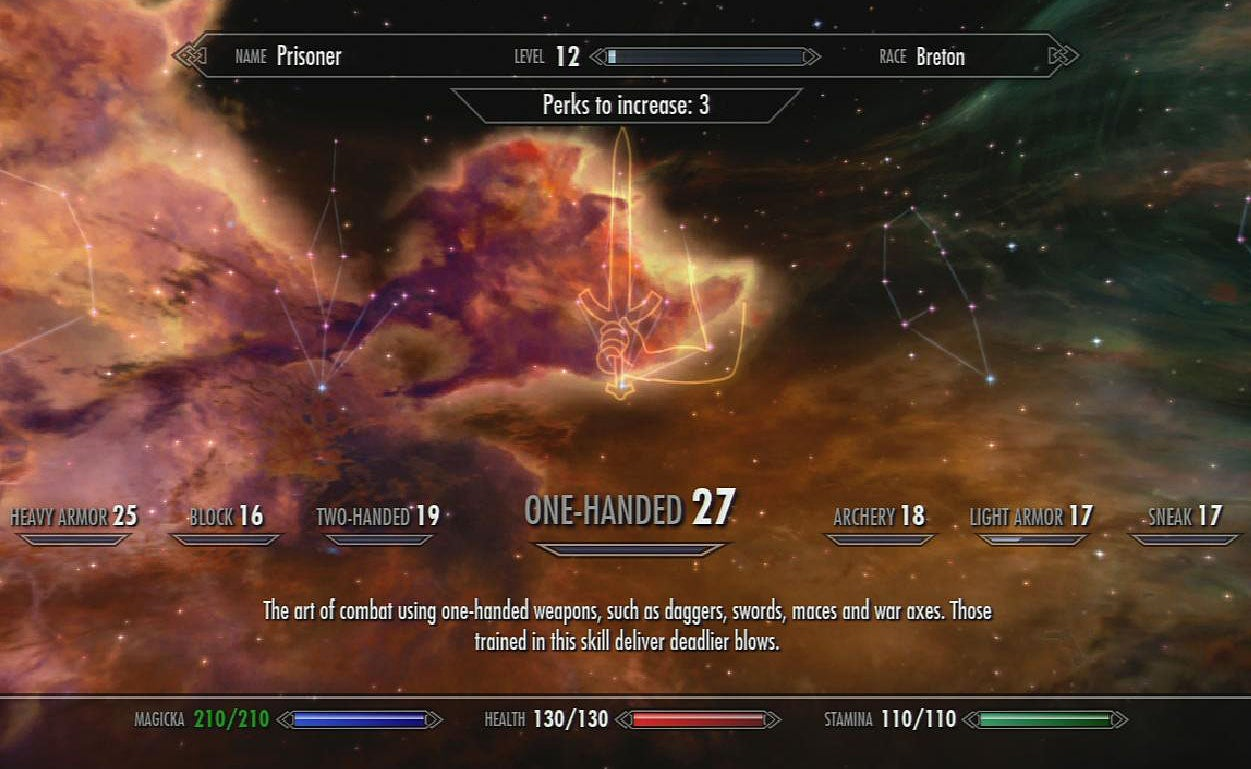
\includegraphics[width=1.0\textwidth]{images/tes.jpg}
\caption{Ekran rozwoju postaci z gry TESV:Skyrim.}
\end{figure}
